
% THIS TEMPLATE IS A WORK IN PROGRESS
% Adapted from an original template by faculty at Reykjavik University, Iceland

\documentclass{scrartcl}

% Adapted from an original template by Hlyni Arnórssyni, Reykjavik University, Iceland
%
% ------------------------------ SETTINGS
\usepackage{geometry}

\geometry{
	paper=a4paper, % Paper size
	top=2.5cm, % Top margin
	bottom=2.5cm, % Bottom margin
	left=2.5cm, % Left margin
	right=2.4cm, % Right margin
	headheight=0.75cm, % Header height
	footskip=1.5cm, % Space from the bottom margin to the baseline of the footer
	headsep=0.75cm, % Space from the top margin to the baseline of the header
	%showframe, % Uncomment to show how the type block is set on the page
}

\usepackage{blindtext}
%-------------------------------- Character encoding ----------------------------
\usepackage[T1]{fontenc}
\usepackage[utf8]{inputenc}

%----------------------------- Mathematics packages from AMS ---------------

\usepackage{amsmath, amsfonts, amsthm, amssymb}
\usepackage{braket, nicefrac}

% ----------- International System of Units
\usepackage{siunitx}

%------------------------------ Lists / numbers -------------------------
\usepackage{enumitem, multicol}

%------------------------------- Figure insertions --------------
\usepackage{graphicx, float}  % Use option [H] to force the placement of a figure
\usepackage{keystroke}
\usepackage{pgfplots}\usepgfplotslibrary{units}\pgfplotsset{compat=1.16}

%------------------------------- Line Spacing --------------
\usepackage{setspace}

%------------------------------- Depth of the ToC --------------
\setcounter{tocdepth}{2}

%%%%%%%%%%%%%%%%%%%%%%%%%% Hyperlink References %%%%%%%%%%%%%%%%%%%%%%%%%%%
\usepackage{hyperref}

%--------------------% Storage Path for images %-----------------%
\graphicspath{{graphics/}{Graphics/}{./}}

%%%%%%%%%%%%%%%%%%%%%%%%%% Environments %%%%%%%%%%%%%%%%%%%%%%%%%%%
\renewenvironment{abstract}{
    \begin{center}
    \textbf{Abstract}
    \vspace{0.5cm}
    \par\itshape
    \begin{minipage}{0.8\linewidth}}{\end{minipage}
    \noindent\ignorespaces
    \end{center}
}

\newenvironment{keywords}{
    \begin{center}
    \textbf{Keywords}
    \vspace{0.5cm}
    \par
    \begin{minipage}{0.8\linewidth}}{\end{minipage}
    \noindent\ignorespaces
    \end{center}
}

\newenvironment{preface}{
    \begin{center}
    \textbf{Preface}
    \vspace{0.5cm}
    \par
    \begin{minipage}{0.8\linewidth}}{\end{minipage}
    \noindent\ignorespaces
    \end{center}
}

\newenvironment{acknowledgements}{
    \begin{center}
    \textbf{Acknowledgements}
    \vspace{0.5cm}
    \par
    \begin{minipage}{0.8\linewidth}}{\end{minipage}
    \noindent\ignorespaces
    \end{center}
}





\begin{document}
%Title of the report, name of coworkers and dates (of experiment and of report).
\begin{titlepage}
	\centering
	\vspace{2cm}
	%%%% COMMENT OUT irrelevant lines among the 3 below
	{\scshape\LARGE Institute For \par}  %if you're a CS major
	{\scshape\LARGE Computing And Research \par}      %if you're a DS major
	\vspace{1cm}
	{\scshape\Large Research Report - Summer 2022\par}
	%{\large \today\par}
	\vfill
	
	%%%% PROJECT TITLE
	{\huge\bfseries Linguistic Discrimination Research And How To Organize Qualitative Data
\par}
	\vfill
	
	%%%% AUTHOR(S)
	{\Large\itshape Lucy Evans \\}\par
	\vspace{1.5cm}

	\vfill
	supervised by\par
	%%%% SUPERVISOR(S)
	Montreal Benesch, \& Kara Becker


	\vfill
% Bottom of the page
\end{titlepage}

\newpage

\vspace{1cm}

\LARGE\begin{acknowledgements}
\LARGE Thank you Montreal Benesch, He Bai, Satchel Petty, Leo Latimer, Parker Scarpa and Kara Becker at Reed College for involving me in the research that you spent your time conducting. I appreciate all the resources you all provided me immensely. Thank you Mark Galassi and the rest of the team behind the Institute for Computing in Research. Finally, thank you Maria De Hoyos for always being eager to help us finish our projects and see our success, I appreciate your help in my application into the institute and I am forever grateful. 
\end{acknowledgements}

\newpage


\LARGE\begin{abstract}
            A team of researchers at Reed College developed a Qualtrics survey to conduct research on linguistic discrimination in a Portland liberal arts college. Using RStudio their research is visualized and easily understandable with the user-friendliness of RStudio and the helpful aspects the program provides.
\end{abstract}
\vspace{1cm}

\newpage



\doublespacing
\tableofcontents
\singlespacing

\newpage

\doublespacing

\section{Introduction}

\MEDIUM Linguistic discrimination is the discrimination against language use, pronunciation, syntax, vocabulary and more. The discrimination against language is prevalent anywhere, but in this paper I will be focused on the study a group of Reedies did on the discrimination of linguistics at their college, and how they used RStudio to visualize the data.

\section{Research Resource Appreciation}

This paper could not have been written without the useful material from the Reed College linguistic researchers. They provided me with multiple pages detailing their research and what they have done up to the 2022 summer, and allowed me to sit in on their meetings to learn more about what their goals were.

\section{Linguistic Discrimination}

Language is common among all beings. We use it to interact with one another, to share our problems and our dreams. Language is the way we connect whether it's spoken, felt, or heard. So, why do we use it as a way to divide one another and discriminate against each other? 

Linguistic discrimination is the discrimination of languages and the way someone communicates. It's a huge epidemic that isn't talked enough about, or at least it isn't mentioned because it benefits some people. Those who speak English, have an "American" accent and or are white all benefit from linguistic discrimination because they are seen as the "norm" when truthfully, there is no norm and language is not supposed to be a way to divide us discriminately. It should be used as a way to appreciate each other and appreciate our differences.

The way you speak can determine by society where you will fit in. A job, a school, a relationship, and opportunity is all dictated by language and the way we use it.

So, how can their be a conduction of data that will show us how a certain set of people have experienced or not experienced language discrimination? And how can it be done in a way that is easy to understand as well as encapsulates the data? 

\section{RStudio: A Useful Tool}

RStudio is an editor for the program R (a coding language) that can be used for accurate and helpful research into qualitative data, statistical analysis and easy to understand answers. My interpretation from the research I have done is that RStudio is great for collaboration work especially when it is paired with GitHub (a repository network) that saves your data in a cloud for easy access within a group.

\begin{figure}
  \centering
  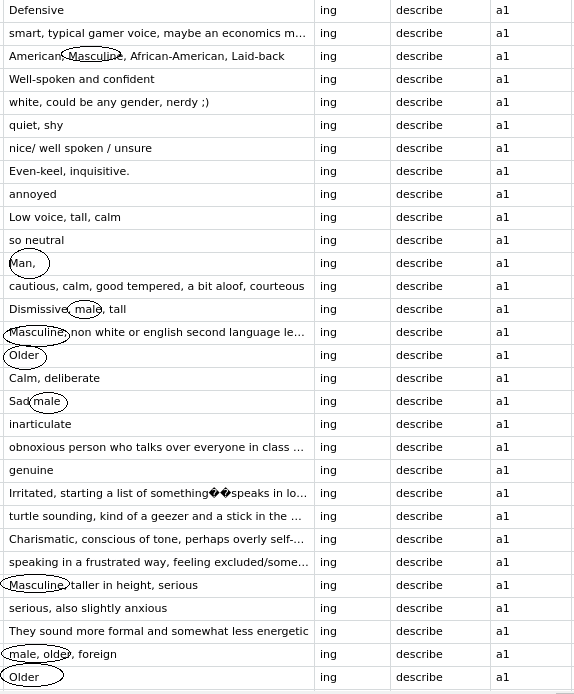
\includegraphics[width=0.5\textwidth]{projectvisual1.png}
  \caption{Survey results}
  \label{fig:survey}
\end{figure}

\section{The Survey}

Using the data from the survey the team at Reed conducted the results were compiled into a spreadsheet like format in RStudio. With over 11,000 cells of data ranging from a rating scale to descriptions of peoples voices. There were many questions with different answers from students and to understand the data and what it was saying each column had to be binned. 

Binning is a method data scientist and statistical researches use to organize data into categories that can produce a clear picture of the message behind the data. 

For example, in the survey like stated before there are multiple speakers and each speaker has a range of different answers from the survey takers. Each adjective that was applied to the voices gets put into different bins depending on what the adjective is. Happy and cheerful would go into a "Bubbly" bin, or "tall" and "6'4" would go into a "Tall" bin. Finding the similarity's between answers is the basis of binning. The differences matter too and can help illustrate the versatility that a voice can bring. 

One person could hear a low voice and assume that that person is tall and male, but another person could hear it and assume the complete opposite. Usually there is a lot of overlap between what listeners describes the voice as. In the study a speaker that talked about their experience at Reed was described multiple times as masculine, male and or older. This doesn't mean that the speaker is any of these things, but it goes to show that their is assumptions by just hearing someones voice. 

\section{Conclusion}
RStudio has many packages that are great for data wrangling like "tidyverse" which has sub-packages like "dplyr" that help organize the data to look prettier. There's a lot that goes into a spreadsheet and because there is so much its nice to be able to clean up the data to lessen the overwhelming amount of it. The more data you have the better your results are and the better the answer to your research question is. That's why RStudio is a must for any kind of research project like the one the linguistic department at Reed did. 


\newpage
\section{References}
\SMALL Bott, Kristin. R Guide for Linguistic Analysis. \par 
https://docs.google.com/document/d/1WDNgzcnZQ_gZFBh1QhGTT \par
-k5tHMP8x4VtlmRh5EYO-s/edit?usp=sharing. \par

---

\SMALL “Data Binning.” Wikipedia, 15 May 2022. Wikipedia, \par
https://en.wikipedia.org/w/index.php?title=oldid=1088054004. \par

---

\SMALL “Linguistic Discrimination.” Wikipedia, 29 June 2022. Wikipedia,\par 
https://en.wikipedia.org/w/index.php?title=Linguistic_discrimination\par
&oldid=1095658038\par

---

“---.” Wikipedia, 29 June 2022. Wikipedia, https://en.wikipedia. \par
org/w/index.php?title=Linguistic_ \par discrimination&oldid=1095658038. \par

---

Quick-R: Pie Charts. https://www.statmethods.net/graphs/pie.html. Accessed 26 July 2022.\par

---

“R Guide for Linguistic Analysis - Master.” Google Docs, \par https://docs.google.com/document/d/1WDNgzcnZQ_gZFBh1QhGTT-k5tHMP8x4VtlmRh5EYO \par
/edit?usp=sharing&usp=embed_facebook.Accessed 26 July 2022.\par

---

“R (Programming Language).” Wikipedia, 17 July 2022. Wikipedia, \par https://en.wikipedia.org/w/index.php?title=R_(programming_language)&oldid=1098779048. \par

---

Reed Lab of Linguistics Team. Lx Diversity and Discrimination. Reed College Linguistic Department, Reed Linguistic Research Team. Summary of What We’ve Been Doing. https://docs.google. \par
com/document/d/1S1Xzrq4ZOKwGpPOxs2NWzmtDc1c \par
7Lkm9dibhHHFxD18/edit.\par

---

“Rename Data Object in R (2 Examples) | Change Name of Vector & List.” Statistics Globe, \par https://statisticsglobe.com/rename-data-object-in-r/. Accessed 26 July 2022. \par

---

“RStudio.” Wikipedia, 19 July 2022. Wikipedia, \par
https://en.wikipedia.org/w/index.php?title=RStudio&oldid=\par
1099226518.\par

---

“RStudio for Dummies.” RStudio Community, 17 Nov. 2018, \par
https://community.rstudio.com/t/rstudio-for-dummies/18403.\par 

---

Split up a String into Pieces. — \par 
Str_split. https://stringr.tidyverse.org/refe \par
rence/str_split.html. Accessed 26 July 2022.\par

\end{document}
